\documentclass[aspectratio=169]{beamer}
\usetheme{Madrid}
\usecolortheme{seahorse}
\usepackage{tikz}
\usepackage{fontawesome5}
\usepackage{amsmath}

% Custom colors for meme aesthetic
\definecolor{memeblue}{RGB}{66, 135, 245}
\definecolor{memepink}{RGB}{255, 105, 180}
\definecolor{cryptogold}{RGB}{255, 193, 7}

\setbeamercolor{palette primary}{bg=memeblue,fg=white}
\setbeamercolor{palette secondary}{bg=memepink,fg=white}
\setbeamercolor{palette tertiary}{bg=cryptogold,fg=black}
\setbeamercolor{structure}{fg=memeblue}

\title{\textbf{FOID.FUN}}
\subtitle{The Debasement Revolution on Fluent Blockchain}
\author{Building the Future of Digital Scarcity}
\date{\today}

\begin{document}

% Title Slide
\begin{frame}
\titlepage
\begin{center}
\Large{\textit{"Not your keys, not your foid"}}
\end{center}
\end{frame}

% Slide 1: ORDINARY WORLD - The Status Quo
\begin{frame}{The Broken NFT Meta}
\framesubtitle{Ordinary World: Where We Started}

\textbf{The Problem:}
\begin{itemize}
\item NFTs are static, boring JPEGs with zero game theory
\item No real scarcity mechanics—just artificial supply caps
\item Communities fade because there's no ongoing engagement
\item No economic consequences to trading behavior
\end{itemize}

\vspace{0.5cm}

\textbf{Meanwhile on Fluent Blockchain:}
\begin{center}
\textit{A new playground for meme culture awaits...}
\end{center}

\end{frame}

% Slide 2: CALL TO ADVENTURE - Enter Foid.Fun
\begin{frame}{Enter the Foid Economy}
\framesubtitle{Call to Adventure: A New Paradigm}

\textbf{What if NFTs had consequences?}

\begin{columns}
\column{0.5\textwidth}
\textbf{Foid Mechanics:}
\begin{itemize}
\item Dynamic NFTs with hidden stats
\item Hot/Crazy Scale (encrypted on-chain)
\item Transfer Tax System (1\% increase per trade)
\item Fertility multipliers
\item Spawning mechanics
\end{itemize}

\column{0.5\textwidth}
\begin{center}
\tikz{
\draw[fill=memepink, draw=memeblue, line width=2pt] (0,0) circle (1.5cm);
\node at (0,0.3) {\Huge \faFemale};
\node at (0,-0.8) {\textbf{FOID}};
}
\end{center}
\end{columns}

\end{frame}

% Slide 3: REFUSAL OF THE CALL - Skepticism
\begin{frame}{Too Degen to Ignore}
\framesubtitle{Refusal: But Is This Too Crazy?}

\textbf{Initial Reactions:}
\begin{itemize}
\item "This is just speculation with extra steps"
\item "Why would anyone want a depreciating asset?"
\item "Meme coins always dump"
\end{itemize}

\vspace{0.5cm}

\textbf{But Consider:}
\begin{center}
\Large{\textcolor{cryptogold}{\textbf{Fiat collapsed. NFTs stagnated. Foids evolve.}}}
\end{center}

\vspace{0.3cm}

The meme is the message. The debasement is the feature.

\end{frame}

% Slide 4: MEETING THE MENTOR - Tokenomics Wisdom
\begin{frame}{The Transfer Tax Revelation}
\framesubtitle{Meeting the Mentor: Understanding True Scarcity}

\textbf{Revolutionary Tax Mechanics:}

\begin{center}
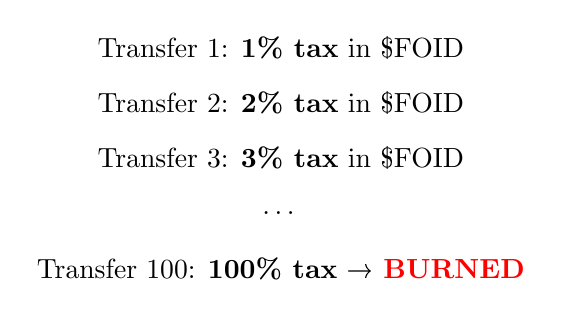
\begin{tikzpicture}
\node at (0,0) {Transfer 1: \textbf{1\% tax} in \$FOID};
\node at (0,-0.7) {Transfer 2: \textbf{2\% tax} in \$FOID};
\node at (0,-1.4) {Transfer 3: \textbf{3\% tax} in \$FOID};
\node at (0,-2.1) {\dots};
\node at (0,-2.8) {Transfer 100: \textbf{100\% tax} → \textcolor{red}{\textbf{BURNED}}};
\end{tikzpicture}
\end{center}

\vspace{0.3cm}

\textbf{The Wisdom:} Every transfer makes your foid more expensive to trade. Paper hands pay the price. Diamond hands accumulate value.

\end{frame}

% Slide 5: CROSSING THE THRESHOLD - Virginity Premium
\begin{frame}{Fresh Foids = Maximum Value}
\framesubtitle{Crossing the Threshold: The Virginity Multiplier}

\textbf{Why Virginity Matters:}

\begin{columns}
\column{0.6\textwidth}
\begin{itemize}
\item \textbf{Zero transfer history} = 0\% tax burden
\item Maximum fertility multiplier
\item Highest spawning probability
\item Pure, untouched on-chain state
\end{itemize}

\vspace{0.3cm}

\textit{"In a world of debasement, virginity is the ultimate store of value"}

\column{0.4\textwidth}
\begin{center}
\Large{\textcolor{memepink}{\textbf{Fertility $\times$ Virginity}}}

\vspace{0.3cm}

\tikz{
\draw[line width=3pt, cryptogold] (0,0) -- (2,2);
\node at (1,-0.5) {Value};
}
\end{center}
\end{columns}

\end{frame}

% Slide 6: TESTS, ALLIES, ENEMIES - The Hot/Crazy Scale
\begin{frame}{Encrypted Chaos}
\framesubtitle{Tests \& Allies: The Hot/Crazy Oracle}

\textbf{Hidden Stats Create Market Inefficiency:}

\begin{center}
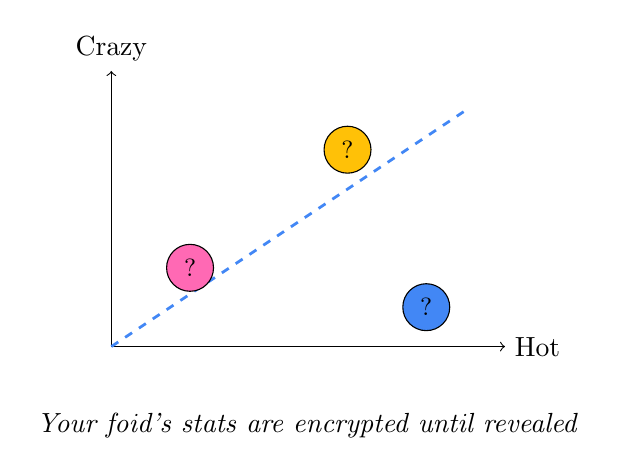
\begin{tikzpicture}
\draw[->] (0,0) -- (5,0) node[right] {Hot};
\draw[->] (0,0) -- (0,3.5) node[above] {Crazy};
\draw[dashed, memeblue, line width=1pt] (0,0) -- (4.5,3);
\node at (3,2.5) [draw, fill=cryptogold, circle] {\small ?};
\node at (1,1) [draw, fill=memepink, circle] {\small ?};
\node at (4,0.5) [draw, fill=memeblue, circle] {\small ?};
\node at (2.5,-1) {\textit{Your foid's stats are encrypted until revealed}};
\end{tikzpicture}
\end{center}

\textbf{Game Theory:}
\begin{itemize}
\item Information asymmetry drives trading
\item Revealing stats = meta shift
\item Crazy high = spawning probability $\uparrow\uparrow$
\end{itemize}

\end{frame}

% Slide 7: APPROACH - Spawning Mechanics
\begin{frame}{Exponential Proliferation}
\framesubtitle{Approach to the Cave: The Spawning Event}

\textbf{How Foids Multiply:}

$$P_{spawn} = f(\text{transfers}) \times \text{fertility} \times \text{crazy\_score}$$

\vspace{0.5cm}

\begin{columns}
\column{0.5\textwidth}
\textbf{Each transfer increases:}
\begin{itemize}
\item Tax burden (\textcolor{red}{$\uparrow$ 1\%})
\item Spawn probability (\textcolor{cryptogold}{$\uparrow\uparrow$})
\item Supply inflation risk
\end{itemize}

\column{0.5\textwidth}
\textbf{New foids are:}
\begin{itemize}
\item Fresh (0\% tax)
\item Random stats
\item Market catalysts
\item Value sinks for \$FOID
\end{itemize}
\end{columns}

\vspace{0.5cm}
\begin{center}
\textit{The more you trade, the more foids flood the market}
\end{center}

\end{frame}

% Slide 8: ORDEAL - The Debasement
\begin{frame}{Hyperinflation by Design}
\framesubtitle{The Ordeal: Fiat-Level Debasement}

\textbf{The Intentional Collapse:}

\begin{center}
\Large{\textcolor{red}{\textbf{We're speedrunning monetary debasement}}}
\end{center}

\vspace{0.5cm}

\begin{itemize}
\item Spawning creates exponential supply growth
\item No cap, no brakes, no mercy
\item \$FOID token captures ALL value flows
\item Meme culture thrives in chaos
\end{itemize}

\vspace{0.5cm}

\textbf{The Beauty:} This isn't a bug. This IS the feature. Every fiat currency dies. We're just doing it in hyperspeed with sick memes.

\end{frame}

% Slide 9: REWARD - The $FOID Token
\begin{frame}{The Value Capture Mechanism}
\framesubtitle{The Reward: \$FOID Token Supremacy}

\textbf{Why \$FOID Wins:}

\begin{center}
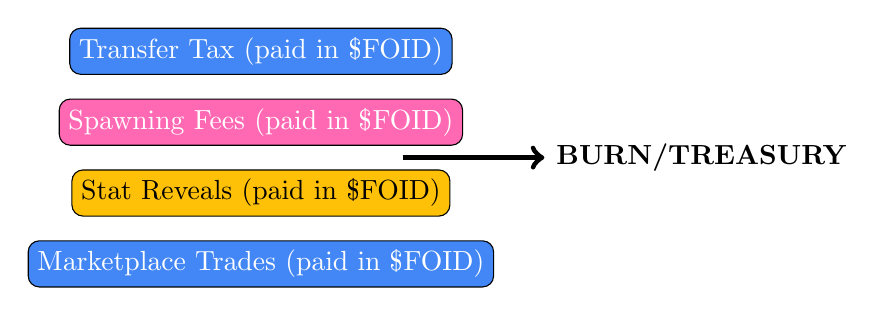
\begin{tikzpicture}[scale=0.9]
\node[draw, fill=memeblue, text=white, rounded corners] at (0,2) {Transfer Tax (paid in \$FOID)};
\node[draw, fill=memepink, text=white, rounded corners] at (0,1) {Spawning Fees (paid in \$FOID)};
\node[draw, fill=cryptogold, rounded corners] at (0,0) {Stat Reveals (paid in \$FOID)};
\node[draw, fill=memeblue, text=white, rounded corners] at (0,-1) {Marketplace Trades (paid in \$FOID)};
\draw[->, line width=2pt] (2,0.5) -- (4,0.5) node[right] {\textbf{BURN/TREASURY}};
\end{tikzpicture}
\end{center}

\vspace{0.3cm}

\textbf{Result:} All economic activity flows through \$FOID. As foid supply explodes, \$FOID becomes the only stable value anchor in the chaos.

\end{frame}

% Slide 10: THE ROAD BACK - Fluent Ecosystem
\begin{frame}{Built on Fluent}
\framesubtitle{The Road Back: Perfect Execution Layer}

\textbf{Why Fluent Blockchain?}

\begin{columns}
\column{0.5\textwidth}
\begin{itemize}
\item High throughput for mass spawning
\item Low fees for meme sustainability  
\item Growing community hungry for innovation
\item Technical capabilities for encrypted state
\end{itemize}

\column{0.5\textwidth}
\begin{center}
\Huge{\textcolor{memeblue}{\faRocket}}

\vspace{0.3cm}

\textit{Fluent + Memes = Culture}
\end{center}
\end{columns}

\vspace{0.5cm}

\textbf{The Magic:} Foid.Fun bootstraps meme culture on Fluent through pure game theory and chaos. No centralized marketing. Just beautiful, algorithmic debasement.

\end{frame}

% Slide 11: RESURRECTION - The Community
\begin{frame}{The Foid Faithful}
\framesubtitle{Resurrection: Community as Moat}

\textbf{What We're Building:}

\begin{itemize}
\item \textbf{Foid Collectors:} Hunting for virgin foids with optimal stats
\item \textbf{Stat Speculators:} Trading on hidden information
\item \textbf{\$FOID Accumulators:} Betting on the token as chaos hedge
\item \textbf{Meme Creators:} Making foid culture irresistible
\item \textbf{Spawning Farmers:} Gaming the proliferation mechanics
\end{itemize}

\vspace{0.5cm}

\begin{center}
\Large{\textcolor{cryptogold}{\textbf{The community doesn't just hold foids...}}}

\textit{They ARE the foids}
\end{center}

\end{frame}

% Slide 12: RETURN WITH ELIXIR - The Vision
\begin{frame}{The New Digital Scarcity}
\framesubtitle{Return with the Elixir: Our Future}

\textbf{What Success Looks Like:}

\begin{enumerate}
\item Foid.Fun becomes THE meme cultural hub on Fluent
\item Debasement mechanics get copied across crypto (we did it first)
\item \$FOID becomes a legitimate chaos hedge asset
\item Virgin foids trade at 100x premiums over used foids
\item The hot/crazy oracle spawns entire derivative markets
\end{enumerate}

\vspace{0.5cm}

\begin{center}
\Huge{\textcolor{memepink}{\faHeart} \textcolor{memeblue}{\faChartLine} \textcolor{cryptogold}{\faFire}}

\vspace{0.3cm}

\Large{\textbf{FOID.FUN}}

\textit{Where debasement meets beauty}
\end{center}

\end{frame}

% Final Slide
\begin{frame}
\begin{center}
\Huge{\textbf{Ready to Collect Foids?}}

\vspace{1cm}

\Large{foid.fun | Built on Fluent}

\vspace{0.5cm}

\textit{The debasement has already begun}

\vspace{1cm}

\faTwitter\ \faDiscord\ \faTelegram
\end{center}
\end{frame}

\end{document}
